\section{Numerical Results}
In this section we illustrate the performance of the discussed metthod through numerical solution of the dissipative wave equation and a port-Hamiltonian model for a dissipative circuit.

\subsection{Dissipative wave equation}

Consider the dissipative linear wave equation
\begin{equation} \label{eq:4.1}
	\begin{aligned}
		q_{t}(t,x) &= p(t,x), \\
		p_{t}(t,x) &= c^2 q_{xx}(t,x) - r(x)  p(t,x) , \\
		q(0,x) &= q_0(x), \\
		p(0,x) &= 0.
	\end{aligned}
\end{equation}
where $x$ belongs to a one-dimensional torus of length $L$ and $r:[0,1]\to[0,1]$ is a positive semi-definite real valued function. 

We discretize the torus into $N_{\Delta x}$ equidistant points and define $\Delta x = L/N_{\Delta x}$, $x_i = i\Delta x$, $q_i=q(t,x_i)$ and $p_i=p(t,x_i)$ for $i = 1, \dots, N_{\Delta x}$. The discretization of $r$ corresponds to a diagonal and semi-positive definite matrix $r_\Delta$. Further, we discretize (\ref{eq:4.1}) using a standard centeral finite differences schemes to obtain
\begin{equation} \label{eq:4.2}
	\dot z = \mathbb J_{2n} K^T K z - R z,
\end{equation}
where $z = (q_1,\dots,q_{N_{\Delta x}},p_1,\dots,p_{N_{\Delta x}})$ and $K$ and $R$ are given as
\begin{equation} \label{eq:4.3}
	K^T K =
	\begin{pmatrix}
		I & 0 \\
		0 & c^2D_x^TD_x
	\end{pmatrix} , \quad
	R =
	\begin{pmatrix}
		0 & 0 \\
		0 & r_\Delta
	\end{pmatrix},
\end{equation}
with $D_x^TD_x = D_{xx}$ the central finite differences matrix operator. Writing (\ref{eq:4.2}) in a TDD formulation gives
\begin{equation} \label{eq:4.4}
\begin{aligned}
	& \dot z = \mathbb J_{2n} K^T f(t) \\
	& f(t) + R \int_0^t f(t) = K z.
\end{aligned}
\end{equation}
Here, since $R$ is not time dependent, it commutes with the integration operator. The Hamiltonian extension of (\ref{eq:4.4}), then takes the form (\ref{eq:2.10.a})-(\ref{eq:2.10.c}).

The initial condition used is given by
\begin{equation} \label{eq:4.5}
	q_i(0) = h( 10\times|x_i - \frac{1}{2}| ), \quad p_i = 0, \quad i=1,\dots,N
\end{equation}
where $h(s)$ is the cubic spline function
\begin{equation} \label{eq:4.6}
h(s) = 
\left\{
\begin{aligned}
& 1 - \frac{3}{2}s^2 + \frac{3}{4}s^3, \quad & 0\leq s \leq 1, \\
& \frac{1}{4}(2-s)^3, & 1< s \leq 2, \\
& 0, & s > 2.
\end{aligned}
\right.
\end{equation}

For the numerical time integration of the extended Hamiltonian system, the Str\"omer-Verlet time stepping scheme (\ref{eq:2.3}) is used. Further in each time step, the system of linear equations (\ref{eq:2.4.1}) is solved to recover $z$. System parameters are summarized below.
\vspace{0.5cm}
\begin{center}
\begin{tabular}{|l|l|}
\hline
Domain length & $L = 1$ \\
No. grid points & $N = 500$ \\
Space discretization size & $\Delta x = 0.002$ \\
Time discretization size & $\Delta t = 0.01$ \\
Wave speed & $c^2 = 0.1$ \\
\hline
\end{tabular}
\end{center}
\vspace{0.5cm}

The first numerical experiment, corresponds to an inhomogeneous dissipative media. Here, $r_{\Delta} = \text{diag}(r_1,\dots,r_{N_{\Delta x}})$, with $r_i = 0.1 + 0.9(i/N_{\Delta x})$, and diag is the MATLAB notation for constructing a diagonal matrix.

Figure \ref{fig:4.1}.a shows the solution of the original dissipative wave equation (\ref{eq:4.1}) at $t \in \{0,2.5,5,7.5\}$. For a nonzero $r_\Delta$ the solution will converge to $(q(t=\infty,x),p(t=\infty,x)) = (\rho,0)$ where $\rho$ is the center of mass of $q_0$. 

To construct the reduced basis for different methods, we gather the snapshots of (\ref{eq:4.1}). We construct RDH reduced system according to the Algorithm \ref{alg:3.1}. The cotangent lift is used to construct an ortho-symplectic reduced basis $A$ (\ref{eq:3.5}). The performance of the RDH method is then compared to the POD, and the method proposed in \cite{peng2016geometric} referred to as the PSD.

Figure \ref{fig:4.1}.b Shows the decay of the singular values of the snapshot matrix for the POD, PSD and the RDH methods. Note that the snapshots for the PSD and the RDH are different since they have different canonical representations. The fast decay of the eigenvalues in all methods is a strong indicator for the existence of a low dimensional reduced system. The reduced bases are then constructed using 20, 40 and 60 number of modes.

The $L^2$ error between the full systems and the RDH, the PSD and the POD method are presented in Figure \ref{fig:4.1}.c. We notice that symplectic methods provide a more accurate solution with respect to the POD method. In fact, the POD method does not yield a stable reduced system.  Further it is seen that enriching the PSD reduced basis does not yield a significant enhancement in the accuracy of the reduced system. This is because in the PSD method, a non-conservative system is being numerically integrated with a symplectic integrator. This results in an incorrect evolution of energy and eventually, in a qualitatively wrong numerical solution.

On the other hand, We notice that the RDH method with 40 modes provides a significantly more accurate solution compared to the PSD method with 60 modes. The RDH method provides a conservative reduced system where the dissipated energy is trapped in the hidden strings. The conservation of energy is then guaranteed using a symplectic integrator. Due to this reason, we observe remarkable increase in the accuracy by enriching the RDH reduced basis.

Figure \ref{fig:4.1}.d shows the preservation of the energy in different methods. The conservation law expressed in theorem \ref{theorem:2.1} is destroyed through the POD model reduction. That is why we observe the blow-up of the system energy. The symplectic methods however, preserves the energy significantly better. Due to the reason discussed above, enriching the PSD basis does not significantly affect the preservation of energy. On the contrary, The RDH not only provides a noteworthy accuracy in preserving the energy, but also provides significant improvement under enrichment.

in Figure \ref{fig:4.1}.e we show the transfer of the energy from the TDD system to the hidden strings, for the full system and the RDH reduced system. We notice that the RDH method preserves the total energy of the extended Hamiltonian system. Further, the transfer of the energy to the hidden strings in the full model is correctly translated in the reduced system.

\begin{figure}[t]
\begin{tabular}{cc}
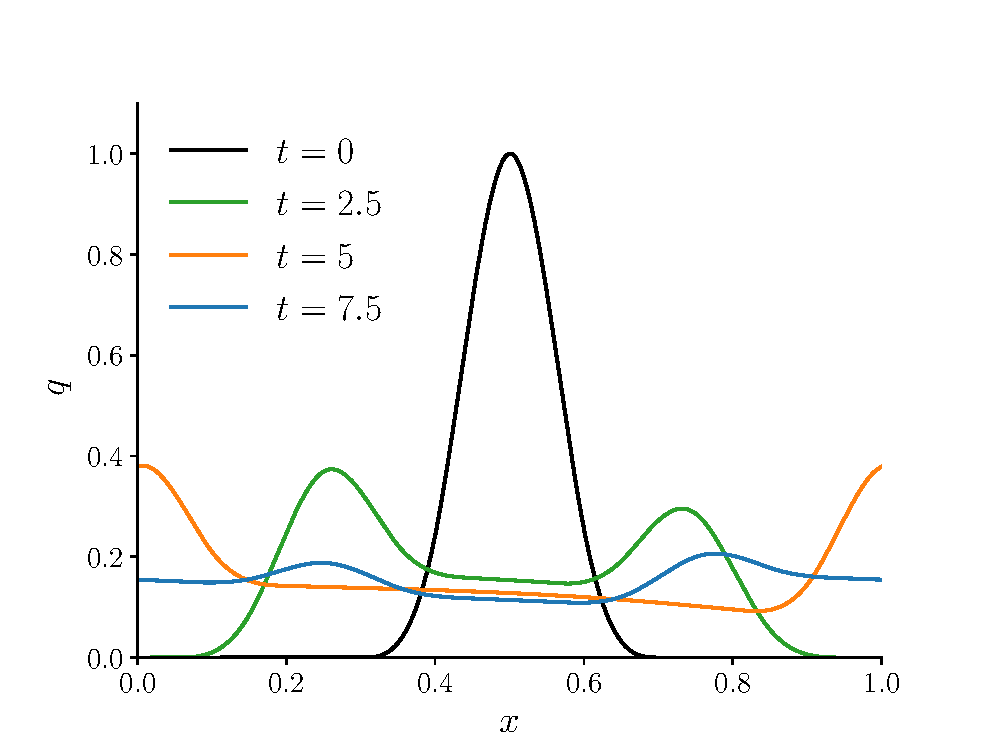
\includegraphics[width=0.5\textwidth]{./figs/wave/solution} & 
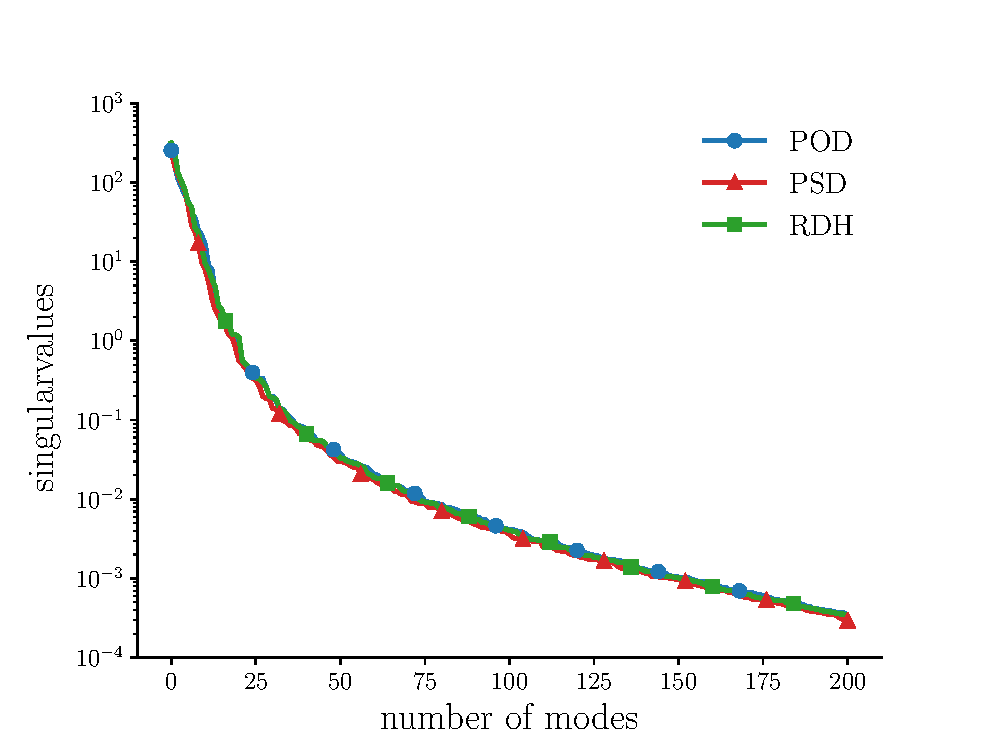
\includegraphics[width=0.5\textwidth]{./figs/wave/singular} \\
(a) & (b) \\
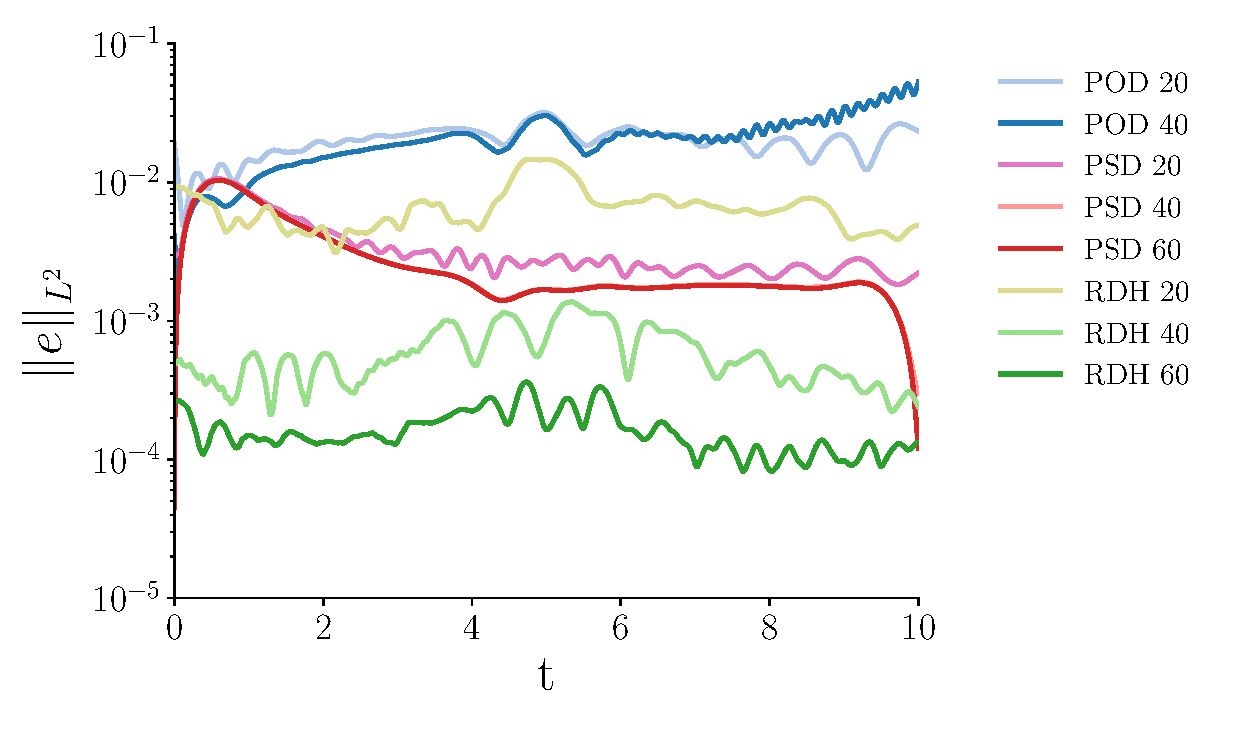
\includegraphics[width=0.5\textwidth]{./figs/wave/error} & 
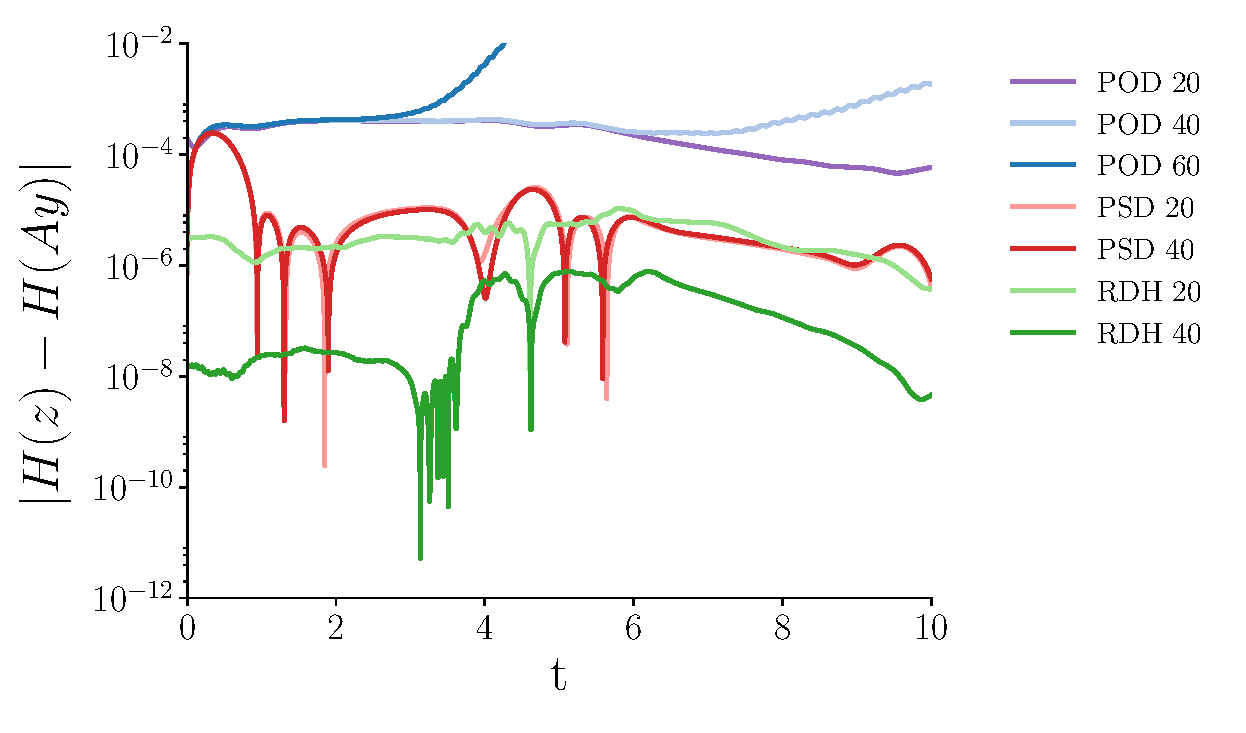
\includegraphics[width=0.5\textwidth]{./figs/wave/energy} \\
(c) & (d) \\
\multicolumn{2} {c} {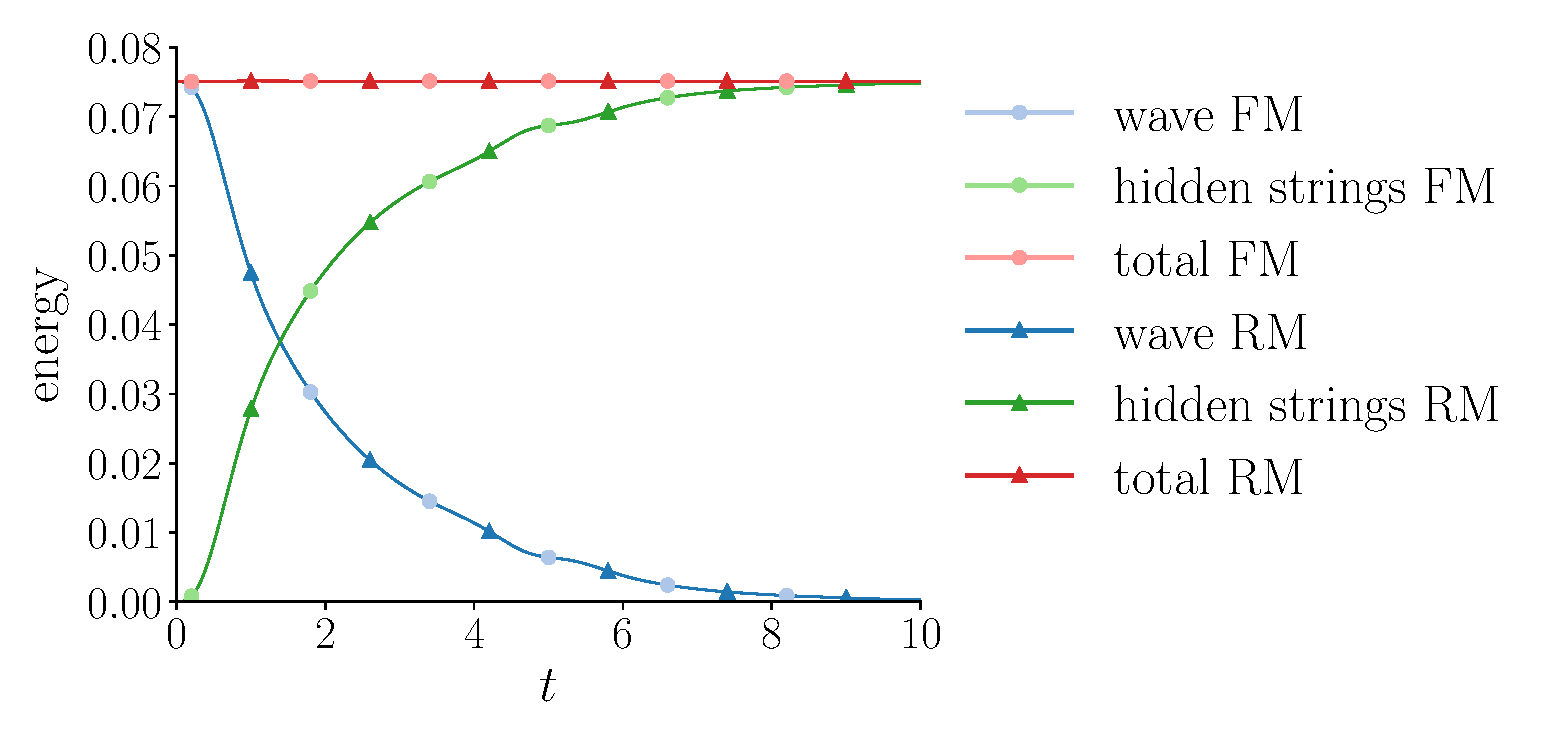
\includegraphics[width=0.7\textwidth]{./figs/wave/energy_conserved}} \\
\multicolumn{2} {c} {(e)} 
\end{tabular}
\caption{(a) The solution to the original dissipative wave equation (\ref{eq:4.1}), (b) The decay of the singular values for the POD, the PSD and the RDH methods, (c) The $L^2$ error for the different methods, (d) Energy preservation for different methods, (e) Energy preservation of the Hamiltonian extension for the original and the reduced system. ``FM'' and ``RM'' stand for the full model and the reduced model respectively.} \label{fig:4.1}
\end{figure}

The second numerical experiment, 
